\question 对给定的关键字序列110,119,007,911,114,120,122进行基数排序,则第2趟分配收集后得到的关键字序列是(
)
\par\fourch{007,110,119,114,911,120,122}{007,110,119,114,911,122,120}{\textcolor{red}{007,110,911,114,119,120,122}}{110,120,911,122,114,007,119}
\begin{solution}基数排序的第1趟排序是按照个位数字来排序的,得到:110,120,911,122,114,007,119。第2趟排序是按照十位数字的大小进行排序的,得到:007,110,911,114,119,120,122。
\end{solution}
\question (华南理工大学,2006年)对各种内部排序方法来说,( )
\par\twoch{快速排序时间性能最佳}{\textcolor{red}{基数排序和归并排序是稳定的排序方法}}{快速排序是一种选择排序}{堆排序使用的辅助空间比较大}
\begin{solution}A快速排序在一定情况下时间复杂度会退化为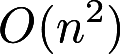
\includegraphics[width=0.43750in,height=0.19792in]{texmath/ead2f65Cdpi7B3507DO28n5E229},B正确,C选择排序即最简单的选出一个最大(最小)数据的排序方式,并非快速排序。D堆排序需要的额外存储空间为O(1),是最小的情况
\end{solution}
